
\documentclass[twocolumn]{article}
\usepackage{mathpazo}
\usepackage{microtype}
\usepackage{times}
\usepackage{titlesec} % 1
%\usepackage{sectsty} % "제 1 절" ...

 %%%%%%%%%%%%%%%%%%%%%%%%%%%%%%%%%%%%%%%%%%%%%%%%%%%%%%%%%%%%%%%%%%%%%%%%%%%%%
 %                              My Commands
\newcommand{\bi}{\begin{itemize}}
\newcommand{\ei}{\end{itemize}}
\newcommand{\be}{\begin{enumerate}}
\newcommand{\ee}{\end{enumerate}}
\newcommand{\ii}{\item}
\newtheorem{Def}{Definition}
\newtheorem{Lem}{Lemma}
\usepackage{algorithm}
\usepackage{algorithmicx}
\usepackage{algpseudocode}

\usepackage{graphicx}
\graphicspath{%
        {converted_graphics/}
        {./images/}
}

\usepackage{color}
\usepackage{xcolor}
\usepackage{listings}
\usepackage{caption}
\DeclareCaptionFont{white}{\color{white}}
\DeclareCaptionFormat{listing}{\colorbox{gray}{\parbox{\textwidth}{#1#2#3}}}
\captionsetup[lstlisting]{format=listing,labelfont=white,textfont=white}
\usepackage{verbatimbox}

\usepackage[hangul,nonfrench,finemath]{kotex}
    
\setlength\textwidth{7in} 
\setlength\textheight{9.5in} 
\setlength\oddsidemargin{-0.25in} 
\setlength\topmargin{-0.25in} 
\setlength\headheight{0in} 
\setlength\headsep{0in} 
%\setlength\columnsep{5pt}
\sloppy 
 
\begin{document}

\title{
\vspace{-0.5in}\rule{\textwidth}{2pt}
\begin{tabular}{ll}\begin{minipage}{4.75in}\vspace{6px}
\noindent\large {\it KIWI Project}@Data Management Research Section\\
\vspace{-12px}\\
\noindent\LARGE ETRI\qquad  \large Technical Report 15ZS1410-TR-65
\end{minipage}&\begin{minipage}{2in}\vspace{6px}\small
218 Gajeong-ro, Yuseong-gu\\
Daejeon, 305-700, South Korea\\
http:/$\!$/www.etri.re.kr/\\
http:/$\!$/sungsoo.github.com/\quad 
\end{minipage}\end{tabular}
\rule{\textwidth}{2pt}\vspace{0.25in}
\LARGE \bf GPU 가속 데이터베이스 기술 조사 \\
\large A Survey on GPU-Accelerated Database Technologies
}

\date{}

\author{
{\bf Sung-Soo Kim}\\
\it{sungsoo@etri.re.kr}
}

\maketitle

\begin{abstract}
모든 산업에서 빅데이터 분석을 통해 기존 산업 영역별 정보화의 새 패러다임을 열어나가고 있다. 
의료 및 헬스케어 산업에서도 예외는 아니다. 미국을 시작으로 기존 의료 및 헬스케어 산업에서는 병원의료정보시스템(HIS, Hospital Information System), 전자의무기록(EMR, Electronic Medical Record), 영상정보관리시스템(PACS, Picture Archiving Communication System), 처방전달시스템(OCS, Order Communication System) 등과 같은 솔루션을 도입해 과거보다 간소화되고 정확해진 워크플로우를 구축하여 활용하고 있다. 
또한, 첨단 의료서비스를 제공하기 위해,  임상데이터웨어하우스 (CDW, Clinical Data Warehouse)를 치료 및 임상 연구 목적으로 적극 활용하고 있다.
하지만, 국내에서는 개인정보 보호법, 개인의료정보 유출우려, 의료정보 활용에 대한 보수적인 시각등으로 빅데이터 기술과 헬스케어 도메인 영역에 대한 적극적인 연계가 현재 답보 상태에 있다. 

과제에서 KIWI 플랫폼을 연계한 서비스로  빅데이터기반 의료데이터 분석 서비스를 목표로 하고 있다.
이와 관련하여 본 기술문서에서는 헬스케어 산업에서 빅데이터 기술을 활용하게 된 배경, 의료/임상 분야의 활동, 관련 연구개발 요소, 그리고 새로운 비즈니스 모델에 대해 논하고자 한다.

\end{abstract}

\section{Introduction}
Bringing intelligent healthcare informatics to bear on the dual problems of reducing healthcare costs and improving quality and outcomes is a challenge even in countries with a reasonably developed technology infrastructure \cite{Hey:2009}. Much of medical knowledge and information remains in paper form, and even where it is digitized, it often resides in disparate datasets and repositories and in diverse formats. Data sharing is uncommon and frequently hampered by the lack of foolproof de-identification for patient privacy. All of these issues impede opportunities for data mining and analysis that would en- able better predictive and preventive medicine.

An era of open information in healthcare is now under way. We have already experienced a decade of progress in digitizing medical records, as pharmaceutical companies and other organizations aggregate years of research and development data in electronic databases. The federal government and other public stakeholders have also accelerated the move toward transparency by making decades of stored data usable, searchable, and actionable by the healthcare sector as a whole. Together, these increases in data liquidity have brought the industry to the tipping point \cite{Groves:2013}.

Healthcare stakeholders now have access to promising new threads of knowledge. This information is a form of  \textit{Big Data}, so called not only for its sheer volume but for its complexity, diversity, and timeliness. 
Pharmaceutical-industry experts, payors, and providers are now beginning to analyze big data to obtain \textit{insights}.
Although these efforts are still in their early stages, they could collectively help the industry address problems related to variability in healthcare quality and escalating healthcare spend. 
For instance, researchers can mine the data to see what treatments are most effective for particular conditions, identify patterns related to drug side effects or hospital readmissions, and gain other important information that can help patients and reduce costs. Fortunately, recent technologic advances in the industry have improved their ability to work with such data, even though the files are enormous and often have different database structures and technical characteristics.

\begin{figure*}[htb]
        \centering
        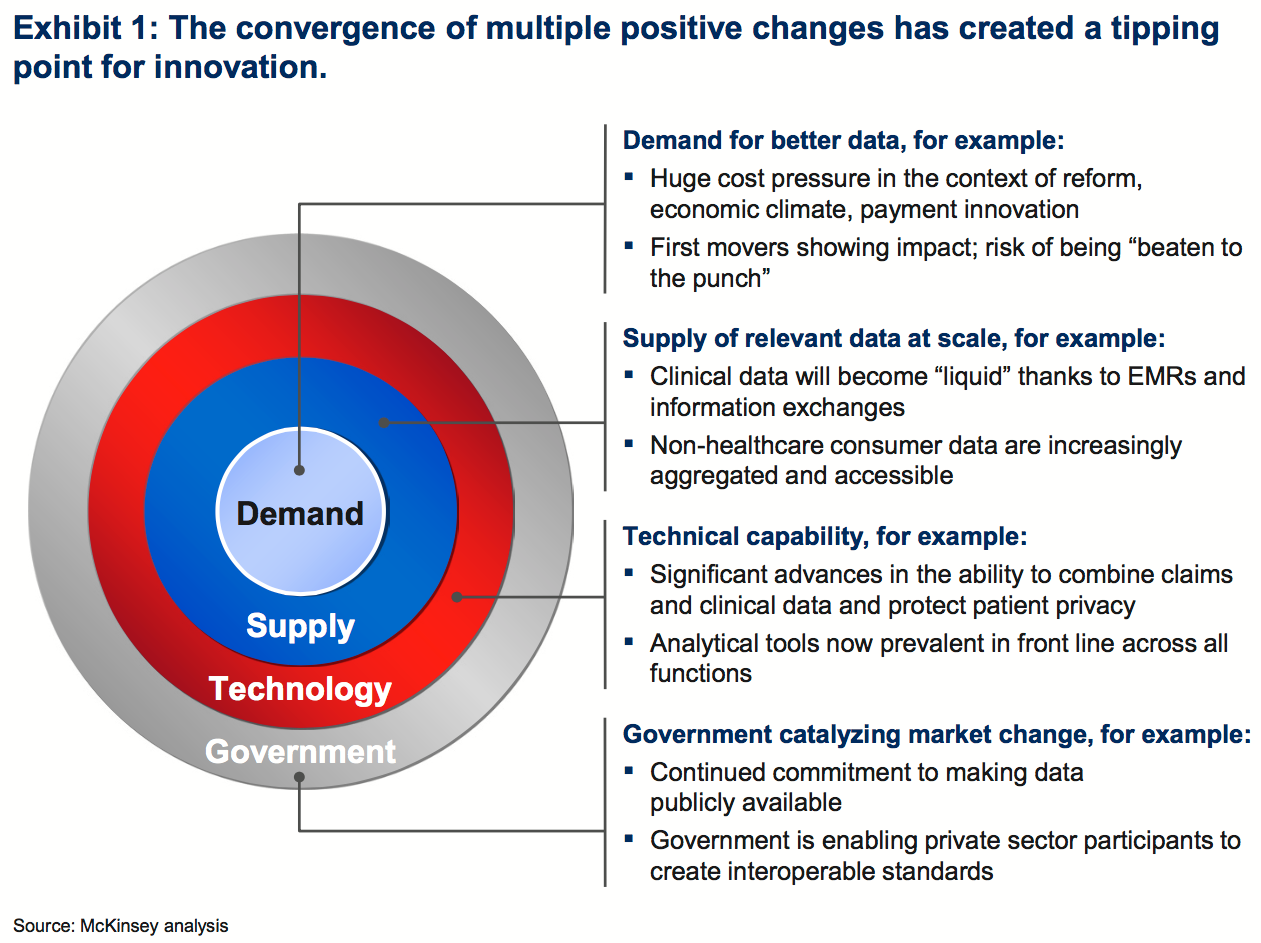
\includegraphics[width=0.7\textwidth]{convergence.png}
        \caption{The convergence of multiple positive changes has created a tipping point for innovation  \cite{Groves:2013}.}
        \label{fig:convergence}
\end{figure*}

Traditionally, the healthcare industry has lagged behind other industries in the use of big data. Part of the problem stems from resistance to change—providers are accustomed to making treatment decisions independently, using their own clinical judgment, rather than relying on protocols based on big data. Other obstacles are more structural in nature. 
Many healthcare stakeholders have underinvested in information technology because of uncertain returns—although their older systems are functional, they have a limited ability to standardize and consolidate data. The nature of the healthcare industry itself also creates challenges: while there are many players, there is no way to easily share data among different providers or facilities, partly because of privacy concerns. And even within a single hospital, payor, or pharmaceutical company, important information often remains siloed within one group or department because organizations lack procedures for integrating data and communicating findings.

But a series of converging trends is now bringing the healthcare industry to a tipping point at which big data can play a major role, as described in Figure \ref{fig:convergence} . 

\section{Clinical Operations}
Within clinical operations are five big data levers that mainly affect the way providers, payors, and pharmaceutical and medical products (PMP) provide clinical care \cite{Manyika:2011}. We estimate that, if fully employed, these five levers could reduce national health care expenditure by up to \$165 billion a year from a base of \$2.5 trillion in 2009.
\subsection{Comparative effectiveness research}
Outcomes-based research determines which treatments will work best for specific patients (“optimal treatment pathways”) by analyzing comprehensive patient and outcome data to compare the effectiveness of various interventions. This research includes what is known as comparative effectiveness research (CER). Many studies have shown that wide variations exist in health care practices, outcomes, and costs across different providers, geographies, and patients. Critically analyzing large datasets that include patient characteristics and the cost and outcomes of treatments can help to identify the most clinically effective and cost-effective treatments to apply. If the health care system implements CER, there is potential to reduce incidences of overtreatment—i.e., interventions that do more harm than good—and undertreatment—cases in which a specific therapy should have been prescribed but was not. Both overtreatment and undertreatment result in worse patient outcomes and higher health care costs in the long run. 

Around the world, agencies such as NICE in the United Kingdom, 
Institute for Quality and Efficiency in Health Care in Germany, the Common Drug Review in Canada, and Australia’s Pharmaceutical Benefits Scheme have begun CER programs with successful results. The United States took a first step in this direction through the American Recovery and Reinvestment Act of 2009. The law created the Federal Coordinating Council for Comparative Effectiveness Research, which, as its name implies, coordinates comparative effectiveness research across the federal government and makes recommendations for the \$400 million allocated for CER. If this lever is to achieve systemwide scale in the United States, it needs to overcome some significant barriers. Comprehensive and consistent clinical and claims datasets need to be captured, integrated,and made available to researchers, and a number of potential issues need to be negotiated. For example, in the current rush to deploy EHR, a potential lack of standards and interoperability could make it difficult to combine datasets. Another concern is how to ensure patient privacy while still providing sufficiently detailed data to allow effective analyses. Having identified optimal treatment pathways, payors will need to be allowed to tie reimbursement decisions and the design of benefits to the results of this research. However, current US law prohibits the Centers for Medicare and Medicaid Services from using the cost/ benefit ratio for reimbursement decisions. Disseminating knowledge about the most effective treatments to medical professionals will require the introduction or upgrade of tools, including clinical decision support systems (see the next lever), so that physicians can receive recommendations of best practices at the point of actual decision making about treatments.

\subsection{Clinical decision support systems}
The second lever is deploying clinical decision support systems for enhancing the efficiency and quality of operations. These systems include computerized physician order-entry capabilities. The current generation of such systems analyzes physician entries and compares them against medical guidelines to alert for potential errors such as adverse drug reactions or events. By deploying these systems, providers can reduce adverse reactions and lower treatment error rates and liability claims, especially those arising from clinical mistakes. In one particularly powerful study conducted at a pediatric critical care unit in a major US metropolitan area, a clinical decision support system tool cut adverse drug reactions and events by 40 percent in just two months.

In the future, big data systems such as these can become substantially more intelligent by including modules that use image analysis and recognition in databases of medical images (X-ray, CT, MRI) for prediagnosis or that automatically mine medical literature to create a medical expertise database capable of suggesting treatment options to physicians based on patients’ medical records. In addition, clinical decision support systems can enable a larger portion of work to flow to nurse practitioners and physician assistants by automating and facilitating the physician advisory role and thereby improving the efficiency of patient care.

\subsection{Transparency about medical data}
The third clinical big data lever is analyzing data on medical procedures and creating transparency around those data both to identify performance opportunities for medical professionals, processes, and institutions and to help patients shop for the care that offers the best value.

\begin{figure*}[htb]
        \centering
        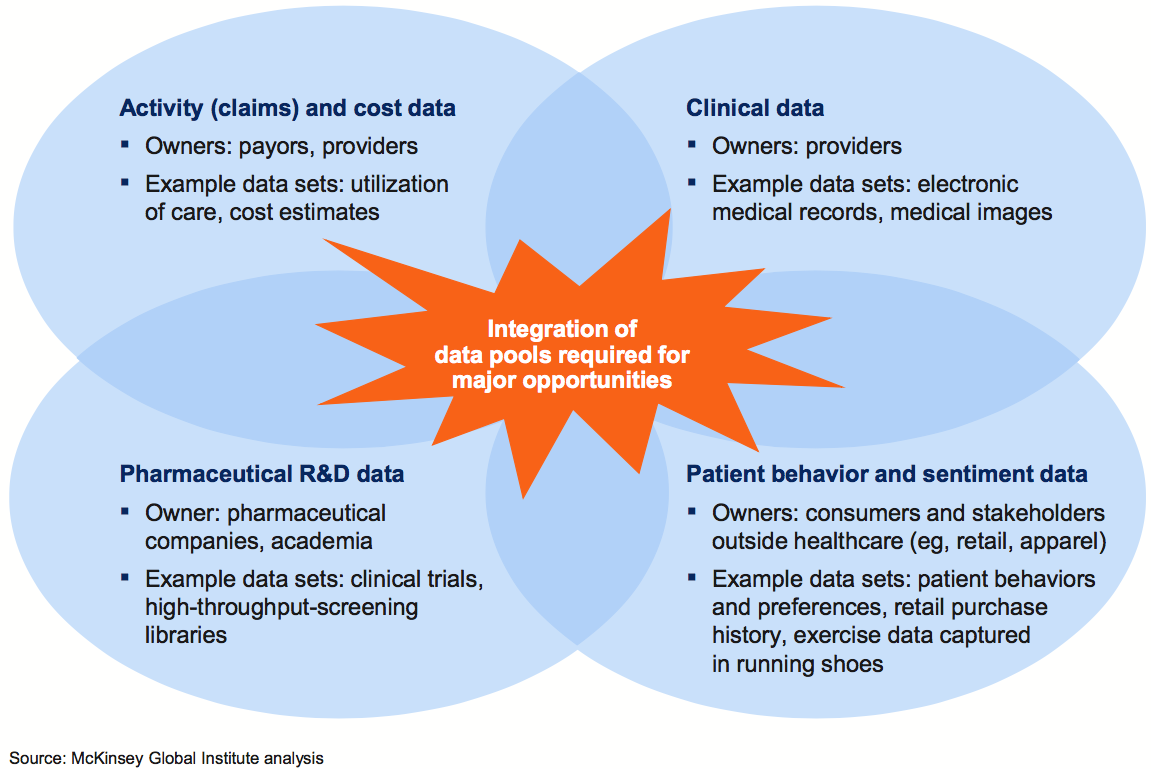
\includegraphics[width=0.7\textwidth]{data-pools.png}
        \caption{Primary data pools are at the heart of the big-data revolution in healthcare \cite{Groves:2013}.}
        \label{fig:data-pools}
\end{figure*}

Operational and performance datasets from provider settings can be analyzed to create process maps and dashboards enabling information transparency. The goal is to identify and analyze sources of variability and waste in clinical processes and then optimize processes. Mapping processes and physical flows as well as "patient journeys" within an organization can help to reduce delays in the system. Simply publishing cost, quality, and performance data, even without a tangible financial reward, often creates the competition that drives improvements in performance. The operational streamlining resulting from these analyses can produce reduced costs through lean processes, additional revenue potential from freed-up capacity, more efficient staffing that matches demand, improved quality of care, and better patient experiences. The Centers for Medicare and Medicaid Services is testing dashboards as part of an initiative to implement open government principles of transparency, public participation, and collaboration. In the same spirit, the Centers for Disease Control and Prevention has begun publishing health data in an interactive format and providing advanced features for manipulating its pretabulated data.

\begin{figure}[htb]
        \centering
        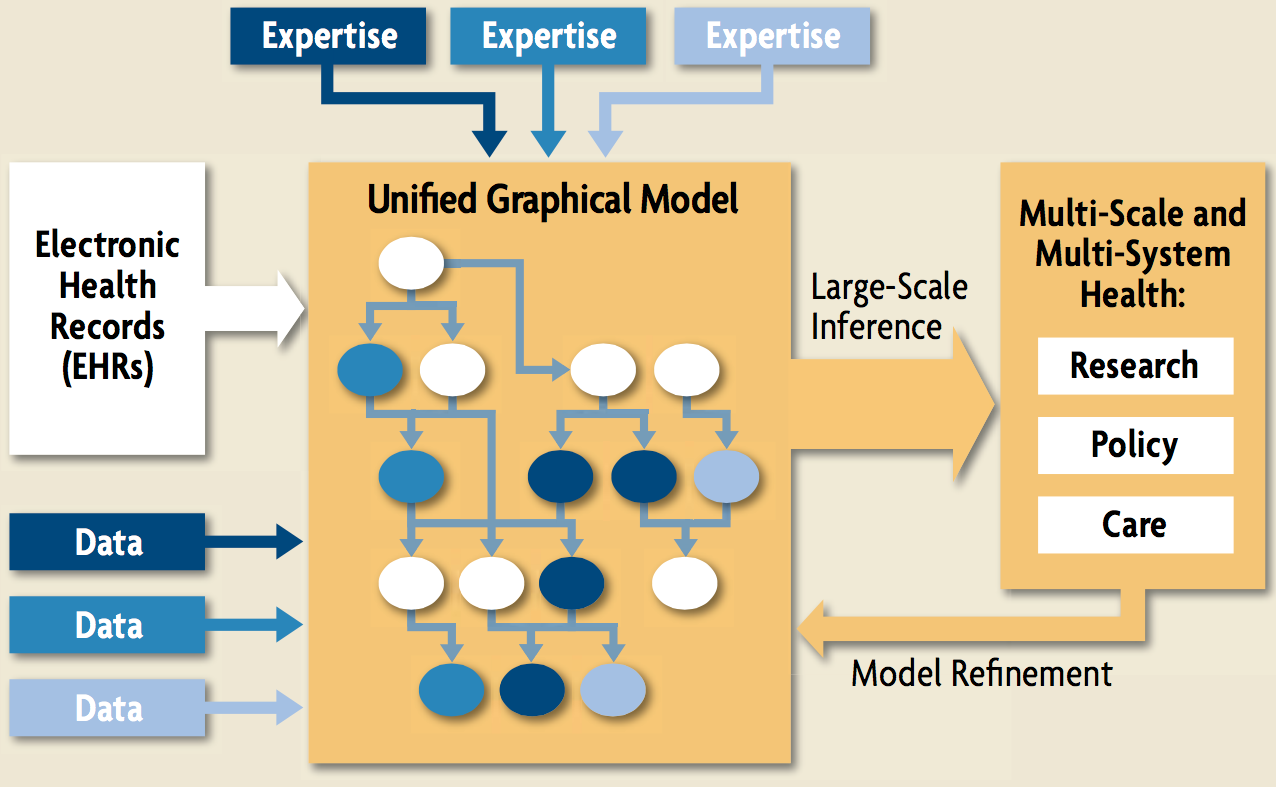
\includegraphics[width=0.5\textwidth]{model.png}
        \caption{A \textit{unified approach} to healthcare modeling that exploits the growing statistical resources of electronic health records in addition to the data collected for specific studies \cite{Hey:2009}.}
        \label{fig:model}
\end{figure}

Publishing quality and performance data can also help patients make more informed health care decisions compared with the situation today in which differences in cost and quality are largely opaque to them.42 Transparency about the data on cost and quality, along with appropriate reimbursement schemes (e.g., where patients’ out-of-pocket expenses are tied to the actual costs charged by the providers) will encourage patients to take a more value-conscious approach to consuming health care, which in turn will help make providers more competitive and ultimately improve the overall performance of the sector.

\subsection{Remote patient monitoring} 
The fourth clinical big data lever is collecting data from remote patient monitoring for chronically ill patients and analyzing the resulting data to monitor adherence (determining if patients are actually doing what was prescribed) and to improve future drug and treatment options. An estimated 150 million patients in the United States in 2010 were chronically ill with diseases such as diabetes, congestive heart failure, and hypertension, and they accounted for more than 80 percent of health system costs that year. Remote patient monitoring systems can be highly useful for treating such patients. The systems include devices that monitor heart conditions, send information about blood-sugar levels, transmit feedback from caregivers, and even include “chip- on-a-pill” technology—pharmaceuticals that act as instruments to report when they are ingested by a patient—that feeds data in near real time to electronic
medical record databases. Simply alerting a physician that a congestive heart failure patient is gaining weight because of water retention can prevent an emergency hospitalization. More generally, the use of data from remote monitoring systems can reduce patient in-hospital bed days, cut emergency department visits, improve the targeting of nursing home care and outpatient physician appointments, and reduce long-term health complications.

\subsection{Advanced analytics applied to patient profiles}
A fifth clinical operations big data lever is applying advanced analytics to patient profiles (e.g., segmentation and predictive modeling) to identify individuals who would benefit from proactive care or lifestyle changes. For instance, these approaches can help identify patients who are at high risk of developing a specific disease (e.g., diabetes) and would benefit from
a preventive care program. These approaches can also enable the better selection of patients with a preexisting condition for inclusion in a disease-management program that best matches their needs. And, of course, patient data can provide an enhanced ability to measure the success of these programs, an exercise that poses a major challenge for many current preventive care programs.

\section{Research and Development}
Five big data levers could improve R\&D productivity in the PMP subsector. 
Together, these levers could create more than \$100 billion in value, about \$25 billion of which could be in the form of lower national health care expenditure.

\begin{figure}[htb]
        \centering
        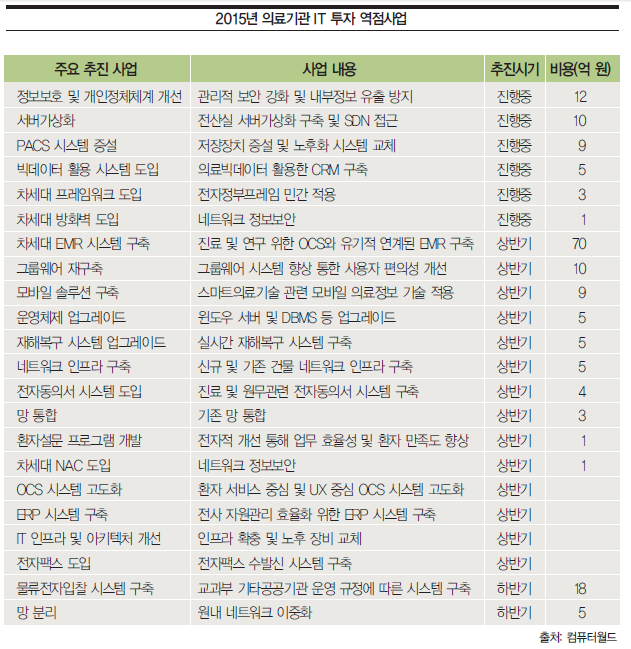
\includegraphics[width=0.5\textwidth]{rnd-korea.png}
        \caption{R\&D projects of clinical institutes in South Korea \cite{Hong:2015}.}
        \label{fig:rnd-korea}
\end{figure}

\subsection{Predictive modeling}
 The first lever is the aggregation of research data so that PMP companies can perform predictive modeling for new drugs and determine the most efficient and cost-effective allocation of R\&D resources. This “rational drug design” means using simulations and modeling based on preclinical or early clinical datasets along the R\&D value chain to predict clinical outcomes as promptly as possible. The evaluation factors can include product safety, efficacy, potential side effects, and overall trial outcomes. This predictive modeling can reduce costs by suspending research and expensive clinical trials on suboptimal compounds earlier in the research cycle.
The benefits of this lever for the PMP sector include lower R\&D costs and earlier revenue from a leaner, faster, and more targeted R\&D pipeline. The lever helps to bring drugs to market faster and produce more targeted compounds with a higher potential market and therapeutic success rate. Predictive modeling can shave 3 to 5 years off the approximately 13 years it can take to bring a new compound to market.

\subsection{Statistical tools and algorithms to improve clinical trial design}
Anotherlever is using statistical tools and algorithms to improve the design of clinical trials and the targeting of patient recruitment in the clinical phases of the R\&D process. This lever includes mining patient data to expedite clinical trials by assessing patient recruitment feasibility, recommending more effective protocol designs, and suggesting trial sites with large numbers of potentially eligible patients and strong track records. The techniques that can be employed include performing scenario simulations and modeling to optimize label size (the range of indications applicable to a given drug) to increase the probability of trial success rates. Algorithms can combine R\&D and trial data with commercial modeling and historic regulatory data to find the optimal trade-off between the size and characteristics of a targeted patient population for trials and the chances of regulatory approval of the new compound. Analyses can also improve the process of selecting investigators by targeting those with proven performance records.

\subsection{Analyzing clinical trials data}
A third R\&D-related lever is analyzing clinical trials data and patient records to identify additional indications and discover adverse effects. Drug repositioning, or marketing for additional indications, may be possible after the statistical analysis of large outcome datasets to detect signals of additional benefits. Analyzing the (near) real-time collection of adverse case reports enables pharmacovigilance, surfacing safety signals too rare to appear in a typical clinical trial or, in some cases, identifying events that were hinted at in the clinical trials but that did not have sufficient statistical power.
These analytical programs can be particularly important in the current context in which annual drug withdrawals hit an all-time high in 2008 and the overall number of new drug approvals has been declining. Drug withdrawals are often very publicly damaging to a company. The 2004 removal of the painkiller Vioxx from the market resulted in around \$7 billion in legal and claims costs for Merck and a 33 percent drop in shareholder value within just a few days.

\begin{figure}[htb]
        \centering
        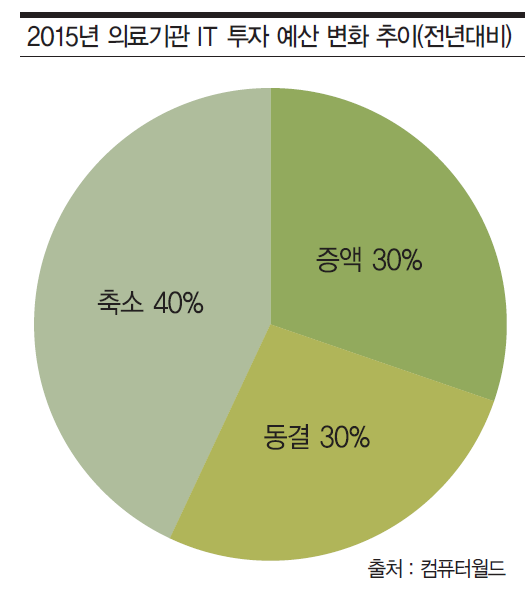
\includegraphics[width=0.35\textwidth]{rnd-trends.png}
        \caption{IT investment budget trends in South Korea \cite{Hong:2015}.}
        \label{fig:budget}
\end{figure}

\subsection{Personalized medicine}
Another promising big data innovation that could produce value in the R\&D arena is the analysis of emerging large datasets (e.g., genome data) to improve R\&D productivity and develop personalized medicine. The objective of this lever is to examine the relationships among genetic variation, predisposition for specific diseases, and specific drug responses and then to account for the genetic variability of individuals in the drug development process.
Personalized medicine holds the promise of improving health care in three main ways: offering early detection and diagnosis before a patient develops disease symptoms; more effective therapies because patients with the same diagnosis can be segmented according to molecular signature matching (i.e., patients with the same disease often don’t respond in the same way to the same therapy, partly because of genetic variation); and the adjustment of drug dosages according to a patient’s molecular profile to minimize side effects and maximize response.
Personalized medicine is in the early stages of development. Impressive initial successes have been reported, particularly in the early detection of breast cancer, in prenatal gene testing, and with dosage testing in the treatment of leukemia and colorectal cancers. We estimate that the potential for cost savings by reducing the prescription of drugs to which individual patients do not respond could be 30 to 70 percent of total cost in some cases. Likewise, earlier detection and treatment could significantly lower the burden of lung cancer on health systems, given that early-stage surgery costs are approximately half those of late-stage treatment.

\subsection{Analyzing disease patterns}
The fifth R\&D-related big data value creation lever is analyzing disease patterns and trends to model future demand and costs and make strategic R\&D investment decisions. This analysis can help PMP companies optimize the focus of their R\&D as well as the allocation of resources including equipment and staff.

\section{New business models}
The proliferation of digital health care data, from clinical to claims information, is creating business models that can complement, or compete with, existing ones and their levers. We highlight two potential new business models:

\subsection{Aggregating and synthesizing patient clinical records and claims datasets}
The first type of new business model is one that aggregates and analyzes patient records to provide data and services to third parties. Companies could build robust clinical datasets that would enable a number of adjacent businesses. These might include licensing and analyzing clinical outcomes data for payors and regulators to improve clinical decision making, leveraging patient databases to help PMP companies identify patients meeting certain criteria for inclusion
in a clinical trial, or providing access to clinical databases for the discovery of biomarkers that help guide the selection of treatments. An adjacent market that is developing not only provides services based on patient clinical records but also integrates claims datasets to provide services to the PMP sector for R\&D and commercial modeling. Clinical and claims data and services markets are just beginning to develop and grow—the rate of their expansion will depend on how rapidly the health care industry implements electronic medical records and evidence-based medicine.

\subsection{Online platforms and communities}
Another potential new business model enabled by big data is that of online platforms and communities, which are already generating valuable data. Examples of this business model in practice include Web sites such as PatientsLikeMe.com, where individuals can share their experience
as patients in the system; Sermo.com, a forum for physicians to share their medical insights; and Participatorymedicine.org, a Web site made available by a nonprofit organization that encourages patient activism. These online platforms could become a valuable source of data. For example, Sermo charges the PMP sector for access to its member physicians and information from their interactions on the site.

\section{Conclusion}
Data alone cannot lead to data-intensive healthcare. A substantial overhaul of methodology is required to address the real complexity of health, ultimately leading to dramatically improved global public healthcare standards. We believe that machine learning, coupled with a general increase in computational thinking about health, can be instrumental.

\bibliographystyle{abbrv}
\bibliography{sqlonhadoop}

\end{document}
